\section{Métodos de inferencia}

La estadística inferencial ofrece dos principales paradigmas para estimar parámetros desconocidos a partir de datos: el enfoque frecuentista y el enfoque bayesiano. Ambos persiguen el mismo objetivo fundamental pero difieren en sus fundamentos filosóficos y metodológicos.

\begin{figure}[h]
\centering
\begin{tikzpicture}[
    node distance=1.5cm and 2cm,
    box/.style={
        draw,
        rounded corners,
        minimum width=2.5cm,
        minimum height=1cm,
        align=center
    },
    arrow/.style={->, thick}
]

% Nodos superiores
\node[box] (sample) {Sample \\ $\mathcal{D}$};
\node[box, right=of sample] (likelihood) {Likelihood \\ $p(\mathcal{D}|\theta)$};

% Nodos del medio
\node[box, below right=1cm and -0.5cm of likelihood] (bayesian) {Bayesian \\ (Prior $p(\theta)$)};
\node[box, below left=1cm and 1cm of likelihood] (frequentist) {Frequentist \\ (No priors)};

% Nodos inferiores
\node[box, below=of frequentist] (estimate) {Estimate $\hat{\theta}$ \\ (e.g. MLE)};
\node[box, below=of bayesian] (posterior) {Posterior \\ $p(\theta|\mathcal{D})$};

% Nodos inferiores finales
\node[box, below=of estimate, minimum width=4cm] (sampling) {Sampling-based Inference \\ (p-values, Confidence Intervals)};
\node[box, below=of posterior, minimum width=3cm] (posterior_inf) {Posterior-\\based Inference};

% Flechas
\draw[arrow] (sample) -- (likelihood);
\draw[arrow] (likelihood) -- (frequentist);
\draw[arrow] (likelihood) -- (bayesian);
\draw[arrow] (frequentist) -- (estimate);
\draw[arrow] (bayesian) -- (posterior);
\draw[arrow] (estimate) -- (sampling);
\draw[arrow] (posterior) -- (posterior_inf);

\end{tikzpicture}
\caption{Comparison between Frequentist and Bayesian inference approaches.}
\label{fig:bayesian_vs_frequentist}
\end{figure}

La Figura \ref{fig:bayesian_vs_frequentist} ilustra las diferencias clave entre estos enfoques. El método frecuentista considera los parámetros como cantidades fijas pero desconocidas, mientras que el enfoque bayesiano los trata como variables aleatorias con distribuciones de probabilidad.

% %%%%%%%%%% 25/08
% \textcolor{red}{Clase: 25/08/205}

Máxima verosimilitud (MLE) es la herramienta principal en la inferencia frecuentista, que busca el valor del parámetro que maximiza la función de verosimilitud dada la muestra observada:

\[x_1,x_2, ..., x_n \rightarrow \theta \]
\[p(x_1, x_2, ..., x_n | \theta) = \prod_{i=1}^{N}p(x_{i} | \theta) \]

En contraste, la inferencia bayesiana utiliza el teorema de Bayes para actualizar la probabilidad de una hipótesis conforme se dispone de más evidencia. Comienza con una distribución a priori que representa nuestras creencias sobre los parámetros antes de observar los datos. Después de observar los datos, actualizamos estas creencias para obtener una distribución posterior, que combina la información previa y la evidencia observada.

La principal diferencia entre ambos enfoques radica en el tratamiento de los parámetros y la incorporación de información previa:

\begin{itemize}
    \item Frecuentista (sin priors): parámetros fijos y desconocidos, estimaciones puntuales.
    \item Bayesiano (con priors): parámetros como variables aleatorias con distribuciones de probabilidad completas.
\end{itemize}


\subsection{Inferencia Bayesiana}

En estadística bayesiana, los parámetros \(\theta\) se tratan como variables aleatorias con sus propias distribuciones de probabilidad. Se comienza con una \textbf{distribución prior} \(p(\theta)\) que representa las creencias sobre \(\theta\) antes de ver los datos. Después de observar los datos \(x\), actualizamos nuestras creencias utilizando el teorema de Bayes \eqref{eq:bayes_theorem}.

\begin{align}
    p(\theta|x) = \frac{p(x|\theta) p(\theta)}{p(x)} \label{eq:bayes_theorem} \\
    p(x) = \int p(x|\theta) p(\theta) d\theta \notag
\end{align}

El posterior \(p(\theta|x)\) combina el conocimiento previo y la evidencia observada.

\(p(x|\theta)\,\rightarrow\) La \textbf{verosimilitud} mide la probabilidad de los datos dados los parámetros, permite cuantificar el nivel de relación entre los datos y los parámetros; cuantifica que tan buenas o malas son las hipótesis.

\(p(\theta)\,\rightarrow\) El \textbf{prior} refleja el conocimiento previo sobre los parámetros antes de observar los datos.

\(p(x)\,\rightarrow\) La \textbf{evidencia} es una constante de normalización que asegura que la distribución posterior sea válida.

\(p(\theta|x)\,\rightarrow\)  El \textbf{posterior} es la distribución actualizada de los parámetros después de observar los datos.

Para que el posterior sea una solución cerrada, el prior y la verosimilitud deben cumplir ciertas condiciones. En muy pocos casos se encuentra que el prior y el likelihood sean gaussianas, por lo que se utilizan métodos numéricos para aproximar el posterior. 

\paragraph{Ejercicio 1.} Dada una muestra \(x_1, x_2, ..., x_n\) que proviene de una distribución Gaussiana con media \(\mu\) y varianza \(\sigma^2\): 

A. Calcular el estimador de máxima verosimilitud para \(\mu\).

B. Suponiendo \(\sigma^2\) conocido, calcular la distribución posterior para \(\mu\) dado un prior Gaussiano \(p(\mu) = \mathcal{N}(\mu_0, \sigma_0^2)\).

\textbf{Solución:}

A. Para calcular el estimador de máxima verosimilitud, primero planteamos la verosimilitud \(p(x_1,x_2, ...,x_n|\theta) = \prod_{i=1}^{n} p(x_i|\mu, \sigma^2)\) dada la muestra observada. Asumimos que las observaciones son independientes e idénticamente distribuidas (i.i.d), por lo que la verosimilitud se puede expresar como el producto de las verosimilitudes individuales:
\[p(AB)=p(A)p(B)\]

Sabiendo que \(\log(AB)=\log(A)+\log(B)\), y dado que es una función monótonamente creciente, podemos maximizar la log-verosimilitud en lugar de la verosimilitud directamente, lo que simplifica los cálculos: 

\[\log p(x_1,x_2, ...,x_n|\mu)=\sum_{i=1}^{N}\log p(x_{i}|\mu)\]

\[\log p(x_1,x_2, ...,x_n|\mu)=\sum_{i=1}^{N}\log \left[\frac{1}{\sqrt{2\pi\sigma^2}}\exp\left(-\frac{(x_i-\mu)^2}{2\sigma^2}\right)\right]
\]
\[\log p(x_1,x_2, ...,x_n|\mu)=\sum_{i=1}^{N}\left[-\frac{1}{2}\log(2\pi\sigma^2)-\frac{(x_i-\mu)^2}{2\sigma^2}\right]\]

Derivando e igualando a cero para encontrar el valor de \(\mu\) que maximiza la log-verosimilitud:
\[\frac{d}{d\mu}\log p(x_1,x_2, ...,x_n|\mu)=\sum_{i=1}^{N}\left[0+\frac{1}{\sigma^2}(x_i-\mu)\right]=0\]
\[\sum_{i=1}^{N}(x_i-\mu)=0\]
\[\sum_{i=1}^{N}x_i-N\mu=0\]
\[\mu=\frac{1}{N}\sum_{i=1}^{N}x_i\]

Por lo tanto, el estimador de máxima verosimilitud para \(\mu\) es la media muestral. El promedio es el estimador de máxima verosimilitud para la media de una distribución Gaussiana.

B. Para calcular la distribución posterior \(p(\mu|x)\) usando el teorema de Bayes \eqref{eq:bayes_theorem}, necesitamos la verosimilitud \(p(x|\mu)\) y el prior \(p(\mu)\).

La verosimilitud para una muestra i.i.d de una distribución Gaussiana es:
\[p(x|\mu) = \prod_{i=1}^{N} p(x_i|\mu) = \prod_{i=1}^{N} \frac{1}{\sqrt{2\pi\sigma^2}} \exp\left(-\frac{(x_i - \mu)^2}{2\sigma^2}\right)\]
\[p(x|\mu) = \left(\frac{1}{\sqrt{2\pi\sigma^2}}\right)^N \exp\left(-\frac{1}{2\sigma^2}\sum_{i=1}^{N}(x_i - \mu)^2\right)\]

El prior Gaussiano es:
\[p(\mu) = \frac{1}{\sqrt{2\pi\sigma_0^2}} \exp\left(-\frac{(\mu - \mu_0)^2}{2\sigma_0^2}\right)\]

Sabiendo que \(\mu\) es una variable aleatoria, calculamos la distribución posterior \(p(\mu|x)\) combinando la verosimilitud y el prior. La expresión para la distribución posterior paso a paso es:
\[p(\mu|x) \propto p(x|\mu)p(\mu)\]
\[p(\mu|x) \propto \left(\frac{1}{\sqrt{2\pi\sigma^2}}\right)^N \exp\left(-\frac{1}{2\sigma^2}\sum_{i=1}^{N}(x_i - \mu)^2\right) \cdot \frac{1}{\sqrt{2\pi\sigma_0^2}} \exp\left(-\frac{(\mu - \mu_0)^2}{2\sigma_0^2}\right)\]
\[p(\mu|x) \propto \exp\left(-\frac{1}{2\sigma^2}\sum_{i=1}^{N}(x_i - \mu)^2 - \frac{(\mu - \mu_0)^2}{2\sigma_0^2}\right)\]

Expandiendo los términos en el exponente:
\begin{align*}
-\frac{1}{2\sigma^2}\sum_{i=1}^{N}(x_i - \mu)^2 - \frac{(\mu - \mu_0)^2}{2\sigma_0^2} &= -\frac{1}{2\sigma^2}\left(\sum_{i=1}^{N}x_i^2 - 2\mu\sum_{i=1}^{N}x_i + N\mu^2\right) \\
&- \frac{1}{2\sigma_0^2}(\mu^2 - 2\mu\mu_0 + \mu_0^2)
\end{align*}

Agrupando los términos en \(\mu^2\), \(\mu\) y los términos constantes:
\[-\frac{1}{2}\left(\frac{N}{\sigma^2} + \frac{1}{\sigma_0^2}\right)\mu^2 + \left(\frac{\sum_{i=1}^{N}x_i}{\sigma^2} + \frac{\mu_0}{\sigma_0^2}\right)\mu + \text{constantes}\]

Completando el cuadrado para expresar el exponente en la forma estándar de una distribución Gaussiana:
\[-\frac{1}{2}\left(\frac{N}{\sigma^2} + \frac{1}{\sigma_0^2}\right)\left(\mu - \frac{\frac{\sum_{i=1}^{N}x_i}{\sigma^2} + \frac{\mu_0}{\sigma_0^2}}{\frac{N}{\sigma^2} + \frac{1}{\sigma_0^2}}\right)^2 + \text{constantes}\]

De esta forma, identificamos que la distribución posterior \(p(\mu|x)\) es una distribución Gaussiana con media y varianza dadas por:
\[\mu_n = \frac{\frac{\mu_0}{\sigma_0^2} + \frac{N\bar{x}}{\sigma^2}}{\frac{1}{\sigma_0^2} + \frac{N}{\sigma^2}}\]
\[\sigma_n^2 = \left(\frac{1}{\sigma_0^2} + \frac{N}{\sigma^2}\right)^{-1}\]

Donde \(\bar{x} = \frac{1}{N}\sum_{i=1}^{N}x_i\) es la media muestral de los datos observados.

Alternativamente, podemos calcular la distribución posterior utilizando la forma logarítmica:


\[\log p(\mu|x)=\log p(x|\mu) + \log p(\mu) - \log p(x)\]

Donde \(p(x)\) es la constante de normalización:
\[p(x)=\int p(x|\mu)p(\mu) d\mu\]

Desarrollando el logaritmo del posterior:
\begin{align*}
\log p(\mu|x) &= -\frac{1}{2}\log(2\pi\sigma^2) - \frac{1}{2}\sum_{i=1}^{N}\frac{(x_i-\mu)^2}{\sigma^2} \\
&-\frac{1}{2}\log(2\pi\sigma_{0}^2) - \frac{1}{2\sigma_{0}^2}(\mu-\mu_{0})^2 + \text{cte.}
\end{align*}

Expandiendo los términos cuadráticos:
\begin{align*}
\log p(\mu|x) &= -\frac{1}{2\sigma^2}\sum_{i=1}^{N}(x_{i}^2-2x_{i}\mu+\mu^2) \\
&-\frac{1}{2\sigma_{0}^2}(\mu^2-2\mu\mu_0+\mu_{0}^2) + \text{cte.}
\end{align*}

Agrupando los términos en \(\mu^2\) y \(\mu\):
\[\log p(\mu|x)=-\frac{1}{2}\left(\frac{N}{\sigma^2}+\frac{1}{\sigma_{0}^2}\right)\mu^2+\left(\frac{\sum_{i=1}^{N}x_i}{\sigma^2}+\frac{\mu_0}{\sigma_0^2}\right)\mu+\text{cte.}\]

Para identificar la distribución posterior como una Gaussiana, comparamos con la forma logarítmica de una distribución normal:
\[\log \mathcal{N}(\bar{\mu},\bar{\sigma^2}) = -\frac{1}{2}\log(2\pi\bar{\sigma^2}) - \frac{(\mu-\bar{\mu})^2}{2\bar{\sigma^2}}\]

Expandiendo:
\[\log \mathcal{N}(\bar{\mu},\bar{\sigma^2}) = -\frac{1}{2}\log(2\pi\bar{\sigma^2}) - \frac{1}{2\bar{\sigma^2}}(\mu^2 - 2\mu\bar{\mu} + \bar{\mu}^2)\]
\[\log \mathcal{N}(\bar{\mu},\bar{\sigma^2}) = -\frac{1}{2\bar{\sigma^2}}\mu^2 + \frac{\bar{\mu}}{\bar{\sigma^2}}\mu + \text{cte.}\]

Comparando los coeficientes con nuestra expresión del posterior, obtenemos:
\[\bar{\sigma^2} = \left(\frac{N}{\sigma^2} + \frac{1}{\sigma_0^2}\right)^{-1}\]
\[\bar{\mu} = \bar{\sigma^2}\left(\frac{\sum_{i=1}^{N}x_i}{\sigma^2} + \frac{\mu_0}{\sigma_0^2}\right) = \frac{\frac{N\bar{x}}{\sigma^2} + \frac{\mu_0}{\sigma_0^2}}{\frac{N}{\sigma^2} + \frac{1}{\sigma_0^2}}\]

Por lo tanto, la distribución posterior \(p(\mu|x)\) es una distribución Gaussiana:
\[p(\mu|x) = \mathcal{N}(\bar{\mu}, \bar{\sigma^2})\]

Esta expresión muestra cómo el posterior combina la información del prior con la de los datos observados, ponderando cada fuente según su precisión relativa. A mayor cantidad de datos (N más grande) o menor varianza en los datos ($\sigma^2$ más pequeña), mayor será el peso asignado a la evidencia empírica. Por otro lado, a menor incertidumbre en el prior ($\sigma_0^2$ más pequeña), mayor será la influencia del conocimiento previo en la estimación final.

La Figura \ref{fig:bayesian_update} ilustra este proceso de actualización bayesiana para un caso específico. En ella podemos observar cómo la distribución prior (línea azul discontinua) con media $\mu_0=2$ y varianza $\sigma_0^2=1.5^2$ se combina con la verosimilitud de los datos (línea roja punteada) que tienen media muestral $\bar{x}=4$ (con N=10 y $\sigma^2=1$) para producir la distribución posterior (línea verde continua) con media $\mu_n=3.7$ y varianza $\sigma_n^2=0.095$.

Este ejemplo ilustra principios clave de la inferencia bayesiana. La media posterior ($\mu_n=3.7$) se encuentra entre la media del prior ($\mu_0=2$) y la media muestral ($\bar{x}=4$), reflejando la influencia combinada del conocimiento previo y los datos. Además, la varianza posterior ($\sigma_n^2=0.095$) es menor que las varianzas del prior y la verosimilitud, mostrando cómo el enfoque bayesiano reduce la incertidumbre al integrar múltiples fuentes de información.
\begin{figure}[htbp]
\centering
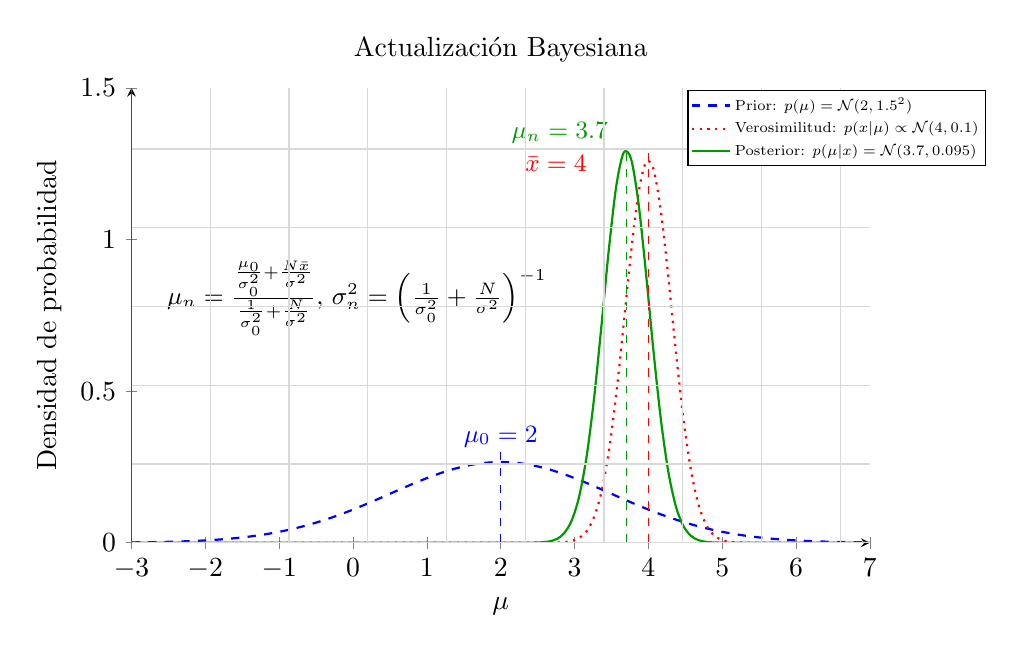
\begin{tikzpicture}
\begin{axis}[
    scale=0.9,
    width=12cm,
    height=8cm,
    axis lines=left,
    xlabel={$\mu$},
    ylabel={Densidad de probabilidad},
    domain=-3:7,
    samples=100,
    smooth,
    title={Actualización Bayesiana},
    legend style={
      at={(0.75,1.0)}, anchor=north west,
      font=\scriptsize,
      nodes={scale=0.75},
      inner sep=1pt, outer sep=1pt,
      legend image post style={xscale=0.8,yscale=0.6}
    },
    legend cell align=left,
    ymax=1.5,
    scaled y ticks=false
]

% Prior - N(2, 1.5²)
\addplot[thick, blue, dashed] {exp(-(x-2)^2/(2*2.25))/sqrt(2*pi*2.25)};
\addlegendentry{Prior: $p(\mu) = \mathcal{N}(2, 1.5^2)$}

% Likelihood basada en datos con media muestral 4, N=10, sigma=1
\addplot[thick, red, dotted] {exp(-(x-4)^2/(2*0.1))/sqrt(2*pi*0.1)};
\addlegendentry{Verosimilitud: $p(x|\mu) \propto \mathcal{N}(4, 0.1)$}

% Posterior - combinación de prior y likelihood
\addplot[thick, green!60!black] {exp(-(x-3.7)^2/(2*0.095))/sqrt(2*pi*0.095)};
\addlegendentry{Posterior: $p(\mu|x) = \mathcal{N}(3.7, 0.095)$}

% Añadir líneas verticales para las medias
\draw[dashed, blue] (axis cs:2,0) -- (axis cs:2,0.3);
\node[blue,font=\small] at (axis cs:2,0.35) {$\mu_0=2$};

\draw[dashed, red] (axis cs:4,0) -- (axis cs:4,1.3);
\node[red,font=\small] at (axis cs:2.75,1.25) {$\bar{x}=4$};

\draw[dashed, green!60!black] (axis cs:3.7,0) -- (axis cs:3.7,1.3);
\node[green!60!black,font=\small] at (axis cs:2.8,1.35) {$\mu_n=3.7$};

% Añadir fórmulas del posterior con posición ajustada
\node[align=left, anchor=south west, font=\small] at (axis cs:-2.65,0.65) {
$\mu_n = \frac{\frac{\mu_0}{\sigma_0^2} + \frac{N\bar{x}}{\sigma^2}}{\frac{1}{\sigma_0^2} + \frac{N}{\sigma^2}}$, 
$\sigma_n^2 = \left(\frac{1}{\sigma_0^2} + \frac{N}{\sigma^2}\right)^{-1}$
};

\draw[gray!30, thin] (axis cs:-3,0) grid (axis cs:7,1.5);

\end{axis}
\end{tikzpicture}
\caption{Actualización bayesiana de la distribución de $\mu$. Ilustra cómo el conocimiento previo (prior) 
se combina con la evidencia (verosimilitud) para obtener la distribución posterior. En este ejemplo, 
asumimos un prior $\mathcal{N}(2, 1.5^2)$, datos con media muestral $\bar{x}=4$ ($N=10$, $\sigma^2=1$), 
resultando en un posterior $\mathcal{N}(3.7, 0.095)$ que se desplaza hacia la evidencia pero con menor varianza que ambas distribuciones originales.}
\label{fig:bayesian_update}
\end{figure}

